Bevor genauer in die Arbeit eingestiegen werden kann, müssen jedoch erstmal die Ausgangssituation dargestellt, ein paar Begriffe geklärt und das Thema etwas abgesteckt werden.

\section{Projektbeschreibung}
Zu Beginn der Arbeit bestand bereits eine Website, die durch einen internen Workshop konzeptioniert und durch ein Pflichtpraktikum implementiert wurde. Die Website wurde mit der Web-Technologie Elixir gebaut, die sowohl Frontend als auch Backend beinhaltet. Hierbei handelt  es sich um eine Plattform, die das Ziel hat, das Verleihen und Leihen innerhalb von Bekanntschaftskreisen zu vereinfachen/ ermöglichen. Hierfür kann jeder Nutzer seine eigenen, verleihbaren Gegenstände auf der Plattform eintragen. Zusätzlich können Nutzer sogenannte Kreise erstellen und zusammen mit Freunden bzw. Familie beittreten. Jeder kann dann die Gegenstände sehen, die in den verschiedenen Kreisen verfügbar sind, in denen er Mitglied ist. Zur Kontaktaufnahme gibt es ein Chatsystem, bei dem sich Leute Nachrichten hin und her schicken können, um den Austausch zu organisieren.

\section{Funktionsumfang der Beispiel Anwendung}
Um den Arbeitsaufwand realistisch zu halten und trotzdem ein generelles Bild abgeben zu können. Werde ich die Implementierung wie folgend beschrieben einschränken.
Allgemein soll eine App gebaut werden, die sich an einer bestehende Webanwendung zum Design orientiert und einen Teil der Funktionalität abbilden soll.
\TODO{Hier irgendwie noch etwas zum Sharingproijekt erklären}
Hierzu kommt zumindest ein Login und Datenspeicherung und Datenabruf um eine Kommunikation mit einem Server zu haben. Außerdem soll es eine grundsätzliche Erklärungsseite mit der möglichkeit zum Login geben. Dazu kommen die Möglichkeit Dinge zu erstellen
\TODO{eventuell wird hier auch noch der Nachtrichtenaustausch hinzugefügt, so könnte man ein Massegesystem auch noch hat}.
Bei den veschiedenen Ansätzen wird immer nur auf eine Plattform näher eingegangen. Dies bedeutet dass bei der nativen und der hybriden Entwicklung lediglich auf die Androidseite eingegangen wird. Dies ist jedoch insofern kein Problem, da die jeweiligen Technologien auch für iOS bestehen und somit nur auf die Entwicklungsumgebung und Programmiersprache angapasst werden müsste. Bei der Cross-Plattform Entwicklung wird lediglich bei der Entwicklung darauf geachtet, dass die App für alle Plattformen kompatibel bleibt. So gesehen kann dann die App auf jeder nötigen Plattform veröffentlicht werden.

Beschränkung auf Willkommenscreen, Login, Ding Anlegen, Ding detail, Eigene Dinge liste, Nachrichtenplattform
Dadurch hat man die in den meisten applikationen notwendigen Funktionalitäten abgedeckt und auch einen gewissen Teil einer App geschrieben. Es wird zwar dann keine eigene Datenbank eingebaut aber externe über API nutzen.


Um mehrere Unterschiedliche Ansätze implementieren zu können, wurde die App, die entwickelt wurde, auf einen bestimmten Funktionsumfang beschränkt. Dieser soll dabei all das enthalten was bei einer typischen Appbenötigt wird. So hat man einfache Informationsseiten, einen Login, eine Authentifizierung, eine gewisse Art von Navigation, eine Listenansicht, eine Art permanente Speicherung von Daten für den Login und eine Kommunikation mit einem Server um Daten zu erhalten, schicken und evtl zu synchronisieren.

In Abbildung \ref{fig:pageflow} Kann man die in Android und Flutter implementierten Abläufe sehen.  

\begin{figure}[ht]
  \centering
  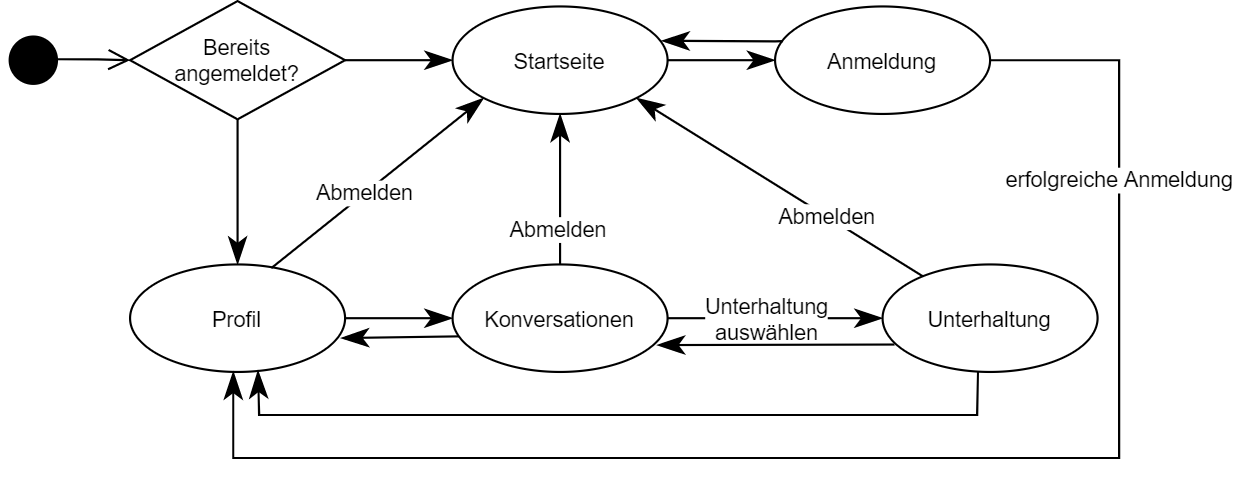
\includegraphics[height=7cm,keepaspectratio]{images/Pageflow_native_flutter.png} 
  \caption{Verbindungen zwischen den Seiten der implementierten Applikation }
  \label{fig:pageflow}
\end{figure}

\section{Themenabgrenzung}
Keine Spiele weil....
Kein iOS weil....


\section{Begriffe}
Wenn in dieser Arbeit von einer App bzw. Applikation geredet wird, so ist hiermit eine Anwendung gemeint, die für mobile Endgeräte, vorallem Smartphones mit den Betriebssystemen Android bzw. iOS gebaut wurden.
Außerdem ist in dieser Arbeit oft die Rede von Multi-Plattform-Anwendungen. Darunter versteht man eine Anwendung, die nicht nur für eine Plattform geschrieben wurde, sondern für mehrere. Das kann etwa die verschiedenen Smartphone Plattformen beinhalten, können aber auch die verschiedenen PC Plattformen mit einbegriffen werden. Eine Anwendung muss dabei auch nicht alle Plattformen beinhalten, sonder kann auch nur zwei Statt Multi-Plattform-Anwendungen wird häufig auch Cross-Plattform-Applikationen als Begriff genutzt, da dies ein in der Industrie häufig benutzter Wortlaut ist. 

\section{Die verschiedenen App Development Framework Klassen}
Wenn man über Applikationsentwicklung für mobile Endgeräte spricht, muss mann zwischen einigen verschiedenen Varianten unterscheiden.
\TODO{Muss auf jeden Fall noch Quellen, noch mehr und umschreiben.}
\subsection{Native Applikationen}
1.Native Apps:
Native Apps sind Applikationen die mit der Plattformspezifischen Programmiersprache für die einzelnen Plattformen entwickeltwerden. Hierbei wird dann in Kotlin für Android oder Swift für iOS sowohl die UI als auch die Logik der App umgesetzt und ist so gesehen ein eigenständiges System, da die dadurch entwickleten Applikationen nur auf der Plattform genutzt werden können, für die sie geschrieben wurden.
Oft verfügen diese Applikationen auch noch über externe Schnitstellen, oder einer Verbindung zu einem Server, um etwa auf Datenhaltung oder andere Dienste zuzugreifen.
Ein Vorteil dieser Art der Entwicklung ist es, dass man sehr gut die verschiedenen Möglichkeiten der jeweiligen Plattform ausnutzen kann. So ist etwa eine Nutzung der Kamera in nativ entwickelten Applikation deutlich einfacher und besser umsetzbar. Dazu kommt, dass man bessere Nutzeroberflächen bauen kann, die auf die mobile Plattform angepasst sind.
Der Nachteil den eine Native Entwicklung jedoch hat ist der Aufwand und die damit verbundenen Kosten. Um für die beiden vorherschenden Plattformen eine Applikation anbieten zu können, braucht man die doppelte Zeit, als wenn man nur eine App entwickelt. Kommt dann noch eine Website und Serveranwendung oder ähnliches hinzu, wird schnell aus einer kleinen Anwendung ein großer Kostenproduzent.
\subsection{Hybride Applikationen}
2. Hybride Apps:
Hybride Apps sind Applikationen die zu gewissen Anteilen aus nativem Code bestehen und zu gewissen Teilen Code, Schnitstellen oder Darstellungen anderer Websiten bzw. Webapplikationen nutzen. Der häufigste Anatz ist es hier, Webappplikationen zu einem gewissen Anteil in einem Frame der Applikation darzustellen und dabei einzelne Seiten durch nativ entwickelte Oberflächen zu ersetzen und die Daten an die Webapplikationen weiter zu geben. 

\subsection{Cross Plattform Applikationen}
3. Cross-Plattform-Apps
Unterscheidung zwischen Webview in App und z.B. Flutter 

\section{Entscheidung zu unterschiedlichen Ansätzen}

------
Schon genauere Erklärung:
Wenn man die Idee zu einer App hat, gibt es die große Frage, wie man nun anfängt und welche Programmiersprache / Framework man wählt. Hierfür gibt es ganz verschiedene Ansätze.  

Jedoch noch grundlegender ist die Frage nach der Plattform. Es gab lange Zeiten in der Applikationsentwicklung, dass nur eine Webversion veröffentlicht wurde. Mittlerweile nutzen jedoch viele Menschen nur noch ihr Smartphone und wollen dementsprechend auch nur mit mobilen Versionen auskommen. Man kann natürlich auch im Web veröffentlichte Applikationen auf dem Handy nutzen, jedoch gibt es hier zwei Sachen, die dazu führen können, dass man eine eigenständige App entwickelt.
1. Eine auf mobile angepasste UI. - Auch wenn es heutzutage in fast jedem Framework und vor allem in den gängigen UI-Frameworks verschiedene Ansätze gibt, die eine recht nutzerfreundliche Version für mobilgeräte anbieten, oder manchmal auch sogar komplett eigenständige Oberflächen für mobil angezeigt werden, so kann es doch sinvoll sein, nochmal extra angepasste UI in Form einer Applikation nativ für die Geräte zu entwickeln. Dadurch kann man gezielt Oberflächen für die Plattformen bauen und dabei auf Plattform eigene Design Unterstützungen zugreifen. Die eine Bedienung um einiges besser machen.
2. Nutzung von Hardwarefunktionalität. -  Ein noch viel wichtigerer Punkt ist es, Funktionalität die mobile Endgeräte anbieten, zu nutzen, die etwa auf einem PC nicht nutzbar sind. Dazu zählen unter anderem GPS-Nutzung, Kamerafunktionalitäten, Bluetooth-Verbindungen,.... Diese können zwar mnanchmal auch durch einen PC geboten sein, jedoch ist es hier nicht gegeben, während man bei einem Smartphone sicher davon ausgehen kann, dass die Kamera genutzt werden kann. So können einige Geschäftsprozesse der Applikationen vereinfacht oder umgestaltet werden, so dass eine Nutzung der Applikation für den Nutzer einfacher wird, bzw. es können auch neue Funktionalitäten daraus ergeben, die es eventuell davor nicht gab.

Wenn nun die Entscheidung getroffen wurde, dass man eine mobile Applikation entwickeln will, so gibt es nun verschiedene Ansätze bzw. Frameworks, die zur Verfügung stehen. Dabei gibt es viele verschiedene Frameworks die auf den ersten Blick das selbe tun, aber doch recht unterschiedlich sein können und unter gewissen Ummständen sich manche besser eignen als andere. 
Eine der ersten Fragen die dabei im Raum steht. Gibt es bereits eine Webversion der Applikation.
Wenn nicht, so kann es von Anfang an spannend sein, ein Framework zu wählen, dass wie Flutter eine Cross-Plattform-Applikation erzeugt, wo auch eine Webversion mit gehostet werden kann.
Falls es bereits eine Webversion geben, so geht der Weg eher in Richtung von Nativen- bzw. Hybriden Applikationen, da meißt nur noch einzelne Teile der Applikation entwickelt werden müssen. Dies ist jedoch auch kein Grund eine Cross-Plattform-Entwicklung auszuschließen, da dadurch nur ein Code geschrieben werden muss um etwa beide vorherschenden mobilen Plattformen abzudecken: iOS und Android.

'''Hier könnte man so ein Art Diagramm machen mit Fragen und dann Entscheidungswegen. So nach dem Motto finde dein Framework zur entwicklung einer mobilen Applikation.'''
